\label{sec:meth}

We consider deterministic models, expressed as simulators, describing the time-evolution of a state $\mathbf{x}_t \in \mathcal{X}$, where we denote application of the simulator iterating the state as $\mathbf{x}_t \gets f(\mathbf{x}_{t-1})$.
A stochastic, additive perturbation to state, denoted $\mathbf{z}_t \in \mathcal{X}$, is applied to induce a distribution over states.
The distribution from which this perturbation is sampled is denoted $p(\mathbf{z}_t | \mathbf{x}_{t-1})$, although, in practice, this distribution is often state independent.
The iterated state is then calculated as $\mathbf{x}_t \gets f(\mathbf{x}_{t-1} + \mathbf{z}_t)$.

However, we consider the case where the simulator can fail for ``invalid'' inputs, denoted by a return value of $\bot$.
Hence the complete definition of $f$ is ${f:\mathcal{X} \rightarrow \left\lbrace \mathcal{X}, \bot \right\rbrace}$.
The region of valid inputs is denoted as ${\mathcal{X}_{A} \subset \mathcal{X}}$, and the region of invalid inputs as ${\mathcal{X}_{R} \subset \mathcal{X}}$, such that ${\mathcal{X}_{A} \sqcup \mathcal{X}_{R} = \mathcal{X}}$, where the boundary between these regions is unknown.
Over the whole support, $f$ defines a many-to-one function, as $\mathcal{X}_R$ maps to $\bot$.
However, the algorithm we derive only requires that $f$ is one-to-one in the accepted region.
This is not uncommon in real simulators, and is satisfied by, for example, ODE models.
We define the random variable $A_t \in \left\lbrace 0, 1 \right\rbrace$ to denote whether the state-perturbation pair does not yield simulator failure and is ``accepted.''

We define the iteration of perturbed deterministic simulator as a rejection sampler, with a well-defined target distribution (\S\ref{sec:meth:rs}).
We use this definition and the assumptions on $f$ to show that we can target the same distribution by learning the state-conditional density of perturbations, conditioned on acceptance (\S\ref{sec:meth:cov}).
We train an autoregressive flow to fit this density (\S\ref{sec:meth:training}), and describe how this can be used in inference, highlighting the ease with which it can be inserted into a particle filter (\S\ref{sec:meth:using-q}).
We empirically show that using this learned proposal distribution in place of the original proposal improves the performance of particle-based state-space inference methods (\S\ref{sec:experiments}).

\subsection{Brittle Simulators as Rejection Samplers}
\label{sec:meth:rs}
The naive approach to sampling from the perturbed system, shown in Algorithm \ref{alg:rs}, is to repeatedly sample from the proposal distribution and evaluate $f$ until the simulator successfully exits.
This procedure defines $A_t = \mathbb{I} \left[ f(\mathbf{x}_{t-1} + \mathbf{z}_t) \neq \bot \right],\ \mathbf{z}_t \sim p(\mathbf{z}_t | \mathbf{x}_{t-1})$, i.e. successfully iterated samples are accepted with certainty.
This incurs significant wasted computation as the simulator must be called repeatedly, with failed iterations being discarded.
The objective of this work is to derive a more efficient sampling mechanism. 

We begin by establishing Algorithm \ref{alg:rs} as a rejection sampler, targeting the distribution over successfully iterated states.
This reasoning is illustrated in Figure~\ref{fig:rs}.
The behavior of $f$ and the distribution $p(\mathbf{z}_t | \mathbf{x}_{t-1})$ implicitly define a distribution over successfully iterated states.
We denote this ``target'' distribution as $\overline{p}(\mathbf{x}_t | \mathbf{x}_{t-1}) = p(\mathbf{x}_t | \mathbf{x}_{t-1}, A_t = 1)$, where the bar indicates that the sample was accepted, and hence places no probability mass on failures.
Note there is no bar on $p(\mathbf{z}_t | \mathbf{x}_{t-1})$, indicating that it is defined before the accept/reject behaviors of $f$ and hence probability mass may be placed on regions that yield failure.
The functional form of $\overline{p}$ is unavailable, and the density cannot be evaluated for any input value.

\begin{algorithm}[t]
 \caption{Iterate brittle simulator, $\overline{p}(\mathbf{x}_t | \mathbf{x}_{t-1})$.}\label{alg:rs}
 \begin{algorithmic}[1]
  \Procedure{IterateSimulator}{$f$, $\mathbf{x}_{t-1}$}
     \State $\mathbf{x}_t \gets \bot$
     \While{$\mathbf{x}_t == \bot$} 
      \If{$q_{\phi}\ \texttt{is trained}$}
      \State $\mathbf{z}_t \sim q_{\phi}(\mathbf{z}_t | \mathbf{x}_{t-1})$ \Comment{Perturb under $q_{\phi}$.} \label{alg:meth:brittle:p}
      \Else
      \State $\mathbf{z}_t \sim p(\mathbf{z}_t | \mathbf{x}_{t-1})$ \Comment{Perturb under $p$.}
      \EndIf
      \State $\mathbf{x}_t \gets f( \mathbf{x}_{t-1} + \mathbf{z}_t)$ \Comment{Iterate simulator.}
     \EndWhile
     \State $\textbf{return}\ \mathbf{x}_t$
  \EndProcedure
 \end{algorithmic}
\end{algorithm}

\begin{figure}[t]
    \centering
    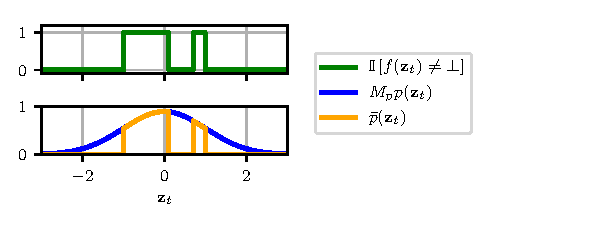
\includegraphics[width=0.45\textwidth]{figures/explanatory-plot.pdf}
    \vspace{-0.3cm}
    \caption{Graphical representation of how a brittle deterministic simulator acts as a rejection sampler, targeting $\overline{p}(\mathbf{z}_t | \mathbf{x}_{t-1})$.
    We set $\mathbf{x}_t = 0$ for clarity.
    The simulator, $f(\mathbf{z}_t)$, returns $\bot$ for unknown input regions, shown in green.
    The proposal over $\mathbf{z}_t$ is shown in blue.
    The target distribution, $\overline{p}(\mathbf{z}_t)$, shown in orange, is implicitly defined as $\overline{p}(\mathbf{z}_t) = \frac{1}{M_p} p(\mathbf{z}_t) \mathbb{I}\left[ f(\mathbf{z}_t) \neq \bot \right]$, where $M_p$ is the normalizing constant from $\overline{p}$, equal to the acceptance rate.
    Accordingly, the proposal distribution, scaled by $M_p$, is \emph{exactly} equal to $\overline{p}(\mathbf{z}_t)$ in the accepted region.
    Algorithm \ref{alg:rs} therefore implicitly constructs a rejection sampler, where the acceptance criterion reduces to $\mathbb{I}\left[ f(\mathbf{z}_t) \neq \bot \right]$, without needing to specify any additional scaling constants.
    }
    \label{fig:rs}
\end{figure}

The existence of $\overline{p}(\mathbf{x}_t | \mathbf{x}_{t-1})$ implies the existence of a second distribution: the distribution over \emph{accepted} perturbations, denoted $\overline{p}(\mathbf{z}_t | \mathbf{x}_{t-1})$.
Note that this distribution is also conditioned on acceptance under the chosen simulator, indicated by the presence of a bar.
We assume $f$ is one-to-one in the accepted region, and so the change of variables rule can be applied to directly relate this to $\overline{p}(\mathbf{x}_t | \mathbf{x}_{t-1})$.
Under our initial algorithm for sampling from a brittle simulator we can therefore write the following identity:
\begin{equation}
\overline{p}(\mathbf{z}_t | \mathbf{x}_{t-1}) = \begin{cases}
      \frac{1}{M_p} p(\mathbf{z}_t | \mathbf{x}_{t-1}), & \text{if}\ f(\mathbf{x}_{t-1} + \mathbf{z}_t)\neq \bot \label{equ:pbarprob}\\
      0, & \text{otherwise}
    \end{cases}
\end{equation}
where the normalizing constant $M_p$ is the acceptance rate under $p$.
\eqref{equ:pbarprob} indicates accepting with certainty perturbations that exit successfully can be seen as proportionally shifting mass from regions of $p$ where the simulator fails to regions where it does not. 
We exploit this definition to learn an efficient proposal.

\subsection{Change of Variable in Brittle Simulator}
\label{sec:meth:cov}
We now derive how we can learn the proposal distribution, denoted $q_{\phi}$ and parameterized by $\phi$, to replace $p$, such that the acceptance rate under $q_{\phi}$ (denoted $M_{q_{\phi}}$) tends towards unity, minimizing wasted computation.
We denote $q_{\phi}$ as the proposal we train, which, coupled with the simulator, implicitly defines a proposal over accepted samples, denoted $\overline{q}_{\phi}$.

Expressing this mathematically, we wish to minimize the distance between joint distribution implicitly specified over \emph{accepted} iterated states using the \emph{a priori} specified proposal distribution, $\overline{p}$, and $\overline{q}_{\phi}$:
\begin{equation}
    \phi^* = \argmin_{\phi} \mathbb{E}_{p(\mathbf{x}_{t-1})} \left[ \mathcal{D}_{\text{KL}} \left[ \overline{p}(\mathbf{x}_t | \mathbf{x}_{t-1}) || \overline{q}_{\phi}(\mathbf{x}_t | \mathbf{x}_{t-1}) \right] \right],\label{equ:sim:target}
\end{equation}
where we select the Kullback-Leibler (KL) divergence as the metric of distance between distributions.
The outer expectation defines this objective as amortized across state space, where we can generate the samples by directly sampling trajectories from the model~\citep{le2016inference, gershman2014amortized}.
We use the forward KL as opposed to the reverse KL, $\mathcal{D}_{\text{KL}} \left[ \overline{q}_{\phi}(\mathbf{x}_t | \mathbf{x}_{t-1}) || \overline{p}(\mathbf{x}_t | \mathbf{x}_{t-1}) \right]$, as high-variance REINFORCE estimators must be used to obtain the the differential with respect to $\phi$ of the reverse KL. 

Expanding the KL term yields:
\begin{align}
\phi^* &= \argmin_{\phi} \mathbb{E}_{p(\mathbf{x}_{t-1})} \mathbb{E}_{\overline{p}(\mathbf{x}_t | \mathbf{x}_{t-1})} \left[ \log\left( w \right) \right], \label{equ:kl_w}\\
w &= \frac{\overline{p}(\mathbf{x}_t | \mathbf{x}_{t-1})}{\overline{q}_{\phi}(\mathbf{x}_t | \mathbf{x}_{t-1})}.
\end{align}
Noting that $\overline{q}_{\phi}$ and $\overline{p}$ are defined only on accepted samples, where $f$ is one-to-one, we can apply a change of variables defined for $\overline{q}_{\phi}$ as:
\begin{equation}
   \overline{q}_{\phi}(\mathbf{x}_t | \mathbf{x}_{t-1}) = \overline{q}_{\phi} ( f^{-1} (\mathbf{x}_{t}) | \mathbf{x}_{t-1})  \left| \frac{\text{d}f^{-1} (\mathbf{x}_{t})}{\text{d}\mathbf{x}_t} \right| , \label{equ:cov_definition}
\end{equation}
and likewise for $p$.
This transforms the distribution over $\mathbf{x}_{t}$ into a distribution over $\mathbf{z}_{t}$ and a Jacobian term:
\begin{align}
w = \frac{\overline{p} (f^{-1} (\mathbf{x}_{t}) | \mathbf{x}_{t-1})  \left| \frac{\text{d}f^{-1} (\mathbf{x}_{t})}{\text{d}\mathbf{x}_t} \right|} {\overline{q}_{\phi} (f^{-1} (\mathbf{x}_{t}) | \mathbf{x}_{t-1})  \left| \frac{\text{d}f^{-1} (\mathbf{x}_{t})}{\text{d}\mathbf{x}_t} \right|}.
\end{align}
taking care to also apply the change of variables in the distribution we are sampling from in \eqref{equ:kl_w}.
Noting that the same Jacobian terms appear in the numerator and denominator we are able to cancel these:
\begin{align}
w = \frac{\overline{p} (f^{-1} (\mathbf{x}_{t}) | \mathbf{x}_{t-1}) } {\overline{q}_{\phi} (f^{-1} (\mathbf{x}_{t}) | \mathbf{x}_{t-1}) }.
\end{align}
We can now discard the $\overline{p}$ term as it is independent of $\phi$.
Noting $f^{-1}(\mathbf{x}_t) = \mathbf{x}_{t-1} + \mathbf{z}_t$ we can write \eqref{equ:sim:target} as:
\begin{align}
\phi^* &=  \argmax_{\phi} \mathbb{E}_{p(\mathbf{x}_{t-1})} \mathbb{E}_{\overline{p}(\mathbf{z}_t | \mathbf{x}_{t-1})} \hspace*{-0.1cm}\left[ \log \overline{q}_{\phi}(\mathbf{z}_t |  \mathbf{x}_{t-1}) \right]\hspace*{-0.1cm}.\label{equ:sim:p_bar_target}
\end{align}
However, this distribution is defined \emph{after} rejection sampling, and can only be defined as in \eqref{equ:pbarprob}:
\begin{align}
    \overline{q}_{\phi}(\mathbf{z}_t | \mathbf{x}_{t-1}) &= q_{\phi}(\mathbf{z}_t | \mathbf{x}_{t-1}, A_t = 1) \\%
    %
    &=  \begin{cases}
    \frac{1}{M_{q_{\phi}}} q_{\phi}(\mathbf{z}_t | \mathbf{x}_{t-1})\ &\text{if}\ f(\mathbf{x}_{t-1} + \mathbf{z}_t) \neq \bot,\\
    0 & \text{otherwise},
    \end{cases}\nonumber
\end{align}
denoting $M_{q_{\phi}}$ as the acceptance rate under $q_{\phi}$.

However, there is an infinite family of $q_{\phi}$ proposals that yield $\overline{p} = \overline{q}_{\phi}$, each a maximizer of \eqref{equ:sim:p_bar_target} but with different rejection rates.
Noting however that there is only a single $q_{\phi}$ that has a rejection rate of zero \emph{and} renders $\overline{q}_{\phi} = \overline{p}$, and that this distribution also renders $q_{\phi} = \overline{q}_{\phi}$, we can instead optimize $q_{\phi}(\mathbf{z}_t | \mathbf{x}_{t-1})$:
\begin{equation}
\phi^* = \argmax_{\phi} \mathbb{E}_{p(\mathbf{x}_{t-1})} \mathbb{E}_{\overline{p}(\mathbf{z}_t  | \mathbf{x}_{t-1})} \left[ \log q_{\phi} ( \mathbf{z}_t | \mathbf{x}_{t-1}) \right],\label{equ:diff_target}
\end{equation}
with no consideration of rejection behavior under $q_{\phi}$.

One might alternatively try to achieve low rejection rates by adding a regularization term to \eqref{equ:sim:p_bar_target} penalizing high $M_{q_{\phi}}$. 
However, differentiation of $M_{q_{\phi}}$ is intractable, meaning direct optimization of \eqref{equ:sim:p_bar_target} is intractable.

The objective stated in \eqref{equ:diff_target} implicitly rewards $q_{\phi}$ distributions that place minimal mass on rejections by placing as much mass on accepted samples as possible.
This expressionn is differentiable with respect to $\phi$ and so we can maximize this quantity through gradient ascent with minibatches drawn from $p(\mathbf{x}_{t-1})$.
This expression shows that we can learn the distribution over accepted $\mathbf{x}_t$ values by learning the distribution over the accepted $\mathbf{z}_t$, \emph{without} needing to calculate the Jacobian or inverse of $f$.
Doing so minimizes wasted computation, targets the same overall joint distribution, and retains interpretability by utilizing the simulator.

\begin{algorithm}[t]
 \caption{Training $q_{\phi}$}\label{alg:meth:training_af}
 \begin{algorithmic}[1]
  \Procedure{TrainQ}{$p(\mathbf{x})$, $\overline{p}(\mathbf{z}_t | \mathbf{x}_{t-1})$, $K$, $N$, $q$, $\phi_0$, $\eta$}
     \For{$k=0:K-1$}
      \For{$n=1:N$}
          \State $\mathbf{x}_{t-1}^{(n)} \sim p(\mathbf{x})$ \Comment{Sample from prior.}
          \State $\mathbf{z}_t^{(n)} \sim \overline{p}(\mathbf{z}_t^{(n)} | \mathbf{x}_{t-1}^{(n)})$ \Comment{Sample noise.}
      \EndFor
      \State $E_k \gets \prod_{n=1}^N q_{\phi_k}\left(\mathbf{z}^{(n)}_{t} | \mathbf{x}^{(n)}_{t-1}\right)$
      \State $\mathbf{G}_k \gets \nabla_{\phi_k} E_k$  \Comment{Do backprop.}
      \State $\phi_{k+1} \gets \phi_k + \eta\left(\mathbf{G}_k\right)$ \Comment{Apply update.}
     \EndFor
     \State $\textbf{return}\ \phi_K$  \Comment{Return learned parameters.}
  \EndProcedure
 \end{algorithmic}
\end{algorithm}

\subsection{Training $q_{\phi}$}
\label{sec:meth:training}
To train $q_{\phi}(\mathbf{z}_t|\mathbf{x}_{t-1})$ we first define a method for sampling state-perturbation pairs.
We initialize the simulator to a state sampled from a distribution over initial value, and then iterate the perturbed simulator forward for some finite period. 
All state-perturbation pairs sampled during the trajectory are treated as a training example, and, in total, represent a discrete approximation to the prior over state for all time, and accepted state-conditional perturbation, i.e. $\mathbf{x}_{t-1} \sim p(\mathbf{x})$ and $\mathbf{z}_{t} \sim \overline{p}(\mathbf{z}_t | \mathbf{x}_{t-1})$.

We train the conditional density estimator $q_{\phi}(\mathbf{z}_t|\mathbf{x}_{t-1})$ using these samples by maximizing the conditional density of the sampled perturbation under the true distribution, as in \eqref{equ:diff_target}, as this minimizes the desired KL divergence originally stated in \eqref{equ:sim:target}. Our conditional density estimator is fully differentiable and can be trained through stochastic gradient ascent as shown in Algorithm~\ref{alg:meth:training_af}. 
The details of the chosen architecture is explained in \S\ref{sec:meth:implementation}.
The result of this procedure is an artifact that approximates the density over valid perturbations conditioned on state, $\overline{p}(\mathbf{z}_t | \mathbf{x}_{t-1})$.

\begin{figure}
    \centering
    % \includegraphics[width=\columnwidth]{figures/p_arch.pdf}
    \includegraphics[width=\columnwidth]{figures/cnf_arch.pdf}
    \caption{Diagram visualizing how $q_{\phi}$ is structured and used. 
    The previous state is input to the hypernetwork, a series of $L$ single layer neural networks, denoted $h_l$.
    Each network outputs parameters, denoted $\phi^l$, for each of the $L$ layers in the flow conditioned on the state.
    The flow samples a perturbation as $\mathbf{z}_t \sim q_{\phi}\left(\mathbf{z}_t | \mathbf{x}_{t-1} \right)$, with the internal states of the flow denoted by $\epsilon_l$.
    This perturbation is summed with the previous state and passed through the simulator, $f$, outputting the iterated state, $\mathbf{x}_t$.
    }
    \label{fig:meth:cnf_arch}
\end{figure}

\subsection{Using $q_{\phi}$}
\label{sec:meth:using-q}
Once $q_{\phi}$ has been trained, it can be deployed to enhance posterior inference, by replacing samples from $p(\mathbf{z}_t | \mathbf{x}_{t-1})$ with $q_{\phi}(\mathbf{z}_t | \mathbf{x}_{t-1})$.
We highlight here the ease with which it can be introduced into an SMC sweep.
The state is iterated by sampling from $\overline{p}(\mathbf{x}_t | \mathbf{x}_{t-1})$ on Line \ref{alg:meth:smc_p:p} of Algorithm \ref{alg:meth:smc_p}, where this sampling procedure is defined in Algorithm \ref{alg:rs}.
Instead of sampling from $p(\mathbf{z}_{t} | \mathbf{x}_{t-1})$ in Algorithm \ref{alg:rs}, the sample is drawn from $q_{\phi}(\mathbf{z}_t | \mathbf{x}_{t-1})$, and as such the sample is more likely to be accepted.
This modification requires only changing a single function call made inside the implementation of Algorithm \ref{alg:rs}.

\subsection{Implementation}
\label{sec:meth:implementation}
We parameterize the density $q_{\phi}$ using an autoregressive flow (AF)~\citep{larochelle2011neural}.
Flows define a parameterized density estimator that can be trained using stochastic gradient descent, and variants have been used in image generation~\citep{kingma2018glow}, as priors for variational autoencoders~\citep{kingma2016improved}, and in likelihood-free inference~\citep{papamakarios2019sequential,lueckmann2019likelihood}.

Specifically, we structure $q_{\phi}$ using a masked autoregressive flow~\citep{papamakarios2017masked}, with $5$ single-layer MADE blocks~\citep{germain2015made}, and batch normalization at the input to each intermediate MADE block.
The dimensionality of the flow is the number of states perturbed in the original model. 
We implement conditioning through the use of a hypernetwork~\citep{ha2016hypernetworks}, which outputs the parameters of the flow layers given $\mathbf{x}_{t-1}$ as input, as shown in Figure \ref{fig:meth:cnf_arch}. 
The hypernetworks are single-layer neural networks defined per flow layer.
Together, the flow and hypernetwork define $q_{\phi}(\mathbf{z}_t|\mathbf{x}_{t-1})$, and can be jointly trained using stochastic gradient descent. 
The networks are implemented in PyTorch~\citep{paszke2017automatic} and are optimized using ADAM~\citep{kingma2014adam}.
